\documentclass[a4paper,10pt]{article}
\usepackage[margin=1in]{geometry}
\usepackage{polski}
\usepackage[utf8x]{inputenc}
\usepackage[unicode]{hyperref}
\usepackage{amssymb}
\usepackage{xifthen}
\usepackage{amsmath}
\usepackage{todonotes}
\usepackage{graphicx}
\usepackage{float}
\usepackage{fullpage}
\usepackage{multirow}
\usepackage{subfig}
\usepackage[europeanresistors,americaninductors]{circuitikz}
\usepackage{tikz}
\usepackage{tikz-3dplot}

%opening
\title{KPub – Manual}
\author{Oskar Świtalski}
\date{}

\begin{document}

\maketitle

\section{Main window}
\begin{figure}[H]
 \centering
 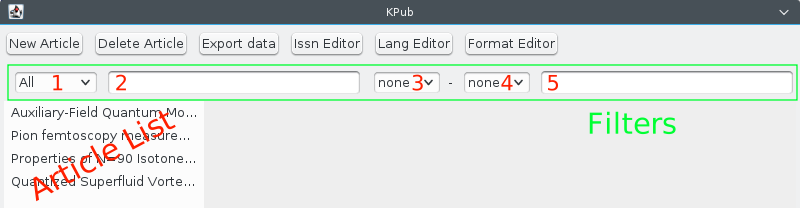
\includegraphics[width=35em]{kpub-main.png}
\end{figure}

\subsection{New Article button}
\paragraph{}Create new article with name 'NEW'.
\subsection{Delete Article button}
\paragraph{}Delete selected article.
\subsection{Export data button}
\paragraph{}Export data to file if file name is *.docx it saves as docx file format, otherwise as plain text file.
\subsection{Issn Editor button}
\paragraph{}Opens \texttt{Issn editior}.
\subsection{Lang Editor button}
\paragraph{}Opens \texttt{Language editior}.
\subsection{Format Editor button}
\paragraph{}Opens \texttt{Format editior}.
\subsection{Filters}
\begin{enumerate}
 \item type
 \item name
 \item form year
 \item to year
 \item authors
\end{enumerate}

\section{Article editor}
\begin{figure}[H]
 \centering
 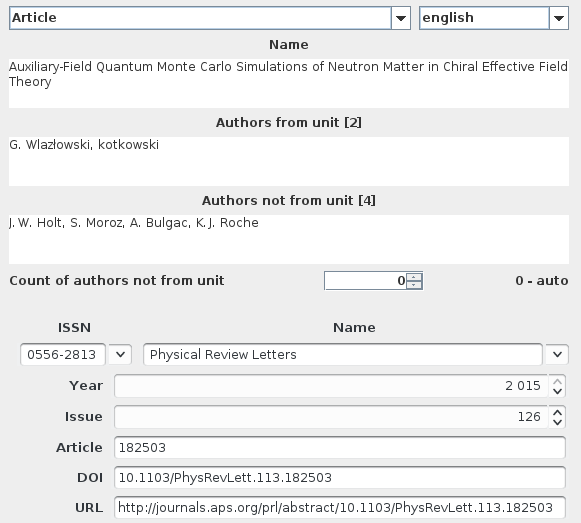
\includegraphics[width=35em]{kpub-article.png}
\end{figure}
\paragraph{Authors} Authors count, between '[' and ']', is callculated using comma and 'and' as separator. Or if count of authors not from unit is not 0, that number is used.
\paragraph{Issn} When ISSN inputed is not found in database it opens \texttt{Issn adder}.

\section{Issn editor}
\begin{figure}[H]
 \centering
 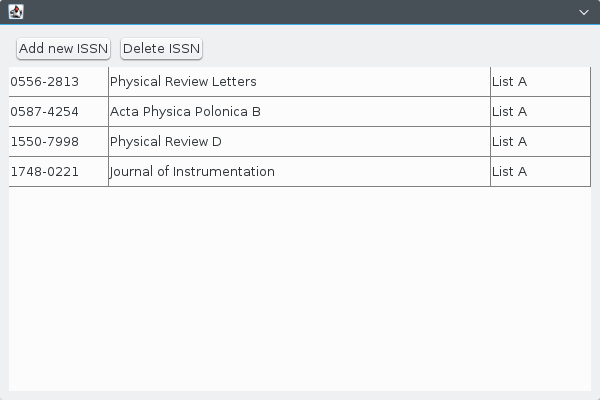
\includegraphics[width=35em]{kpub-issn-editor.png}
\end{figure}
\paragraph{}All fields are editable.
\subsection{Add new Issn}
\paragraph{}Open \texttt{Issn adder}.
\subsection{Delete ISSN}
\paragraph{}Delete selected ISSN.

\section{Issn adder}
\begin{figure}[H]
 \centering
 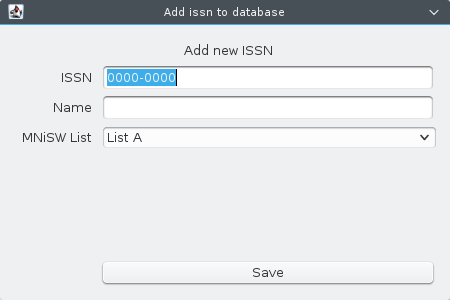
\includegraphics[width=35em]{kpub-issn-add.png}
\end{figure}
\paragraph{}Add new ISSN to database, checks if check sum is correct. Name is journal title.

\section{Language editor}
\begin{figure}[H]
 \centering
 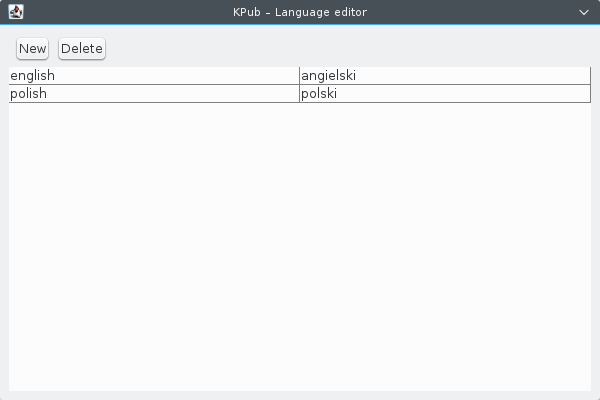
\includegraphics[width=35em]{kpub-lang.png}
\end{figure}
\paragraph{}All fields are editable.
\subsection{New}
\paragraph{}Add new language.
\subsection{Delete}
\paragraph{}Delete selected language.

\section{Format editor}
\begin{figure}[H]
 \centering
 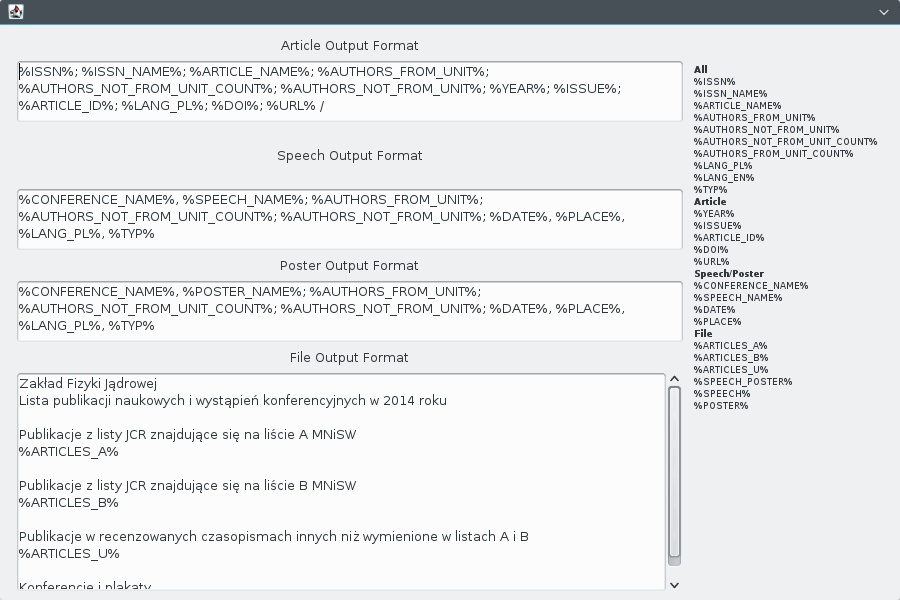
\includegraphics[width=35em]{kpub-format.png}
\end{figure}
\paragraph{}Below are listed possible sequences which will be converted into corresponding variables.
\subsection{Article Output Format}
\begin{itemize}
\item \%ARTICLE\_NAME\% 
\item \%AUTHORS\_FROM\_UNIT\%
\item \%AUTHORS\_NOT\_FROM\_UNIT\%
\item \%AUTHORS\_NOT\_FROM\_UNIT\_COUNT\%
\item \%AUTHORS\_FROM\_UNIT\_COUNT\% 
\item \%LANG\_PL\%
\item \%LANG\_EN\% 
\item \%TYP\%
\item \%ISSN\%
\item \%ISSN\_NAME\%
\item \%YEAR\%
\item \%ISSUE\%
\item \%ARTICLE\_ID\%
\item \%DOI\%
\item \%URL\%
\end{itemize}
\subsection{Speech/Poster Format}
\begin{itemize}
\item \%AUTHORS\_FROM\_UNIT\%
\item \%AUTHORS\_NOT\_FROM\_UNIT\%
\item \%AUTHORS\_NOT\_FROM\_UNIT\_COUNT\%
\item \%AUTHORS\_FROM\_UNIT\_COUNT\% 
\item \%LANG\_PL\%
\item \%LANG\_EN\% 
\item \%TYP\%
\item \%CONFERENCE\_NAME\%
\item \%SPEECH\_NAME\%
\item \%DATE\%
\item \%PLACE\% 
\end{itemize}
\subsection{File Output Format}
\begin{itemize}
\item \%ARTICLES\_A\% – articles from List A
\item \%ARTICLES\_B\% – articles from List B
\item \%ARTICLES\_U\% – articles not listed on List A and B
\item \%SPEECH\_POSTER\% – all speeches and posters
\item \%SPEECH\% – all speeches
\item \%POSTER\% – all posters
\end{itemize}

\end{document}
